% Options for packages loaded elsewhere
\PassOptionsToPackage{unicode}{hyperref}
\PassOptionsToPackage{hyphens}{url}
%
\documentclass[
]{article}
\usepackage{lmodern}
\usepackage{amssymb,amsmath}
\usepackage{ifxetex,ifluatex}
\ifnum 0\ifxetex 1\fi\ifluatex 1\fi=0 % if pdftex
  \usepackage[T1]{fontenc}
  \usepackage[utf8]{inputenc}
  \usepackage{textcomp} % provide euro and other symbols
\else % if luatex or xetex
  \usepackage{unicode-math}
  \defaultfontfeatures{Scale=MatchLowercase}
  \defaultfontfeatures[\rmfamily]{Ligatures=TeX,Scale=1}
\fi
% Use upquote if available, for straight quotes in verbatim environments
\IfFileExists{upquote.sty}{\usepackage{upquote}}{}
\IfFileExists{microtype.sty}{% use microtype if available
  \usepackage[]{microtype}
  \UseMicrotypeSet[protrusion]{basicmath} % disable protrusion for tt fonts
}{}
\makeatletter
\@ifundefined{KOMAClassName}{% if non-KOMA class
  \IfFileExists{parskip.sty}{%
    \usepackage{parskip}
  }{% else
    \setlength{\parindent}{0pt}
    \setlength{\parskip}{6pt plus 2pt minus 1pt}}
}{% if KOMA class
  \KOMAoptions{parskip=half}}
\makeatother
\usepackage{xcolor}
\IfFileExists{xurl.sty}{\usepackage{xurl}}{} % add URL line breaks if available
\IfFileExists{bookmark.sty}{\usepackage{bookmark}}{\usepackage{hyperref}}
\hypersetup{
  pdftitle={hw\_08},
  pdfauthor={Barbara Klein},
  hidelinks,
  pdfcreator={LaTeX via pandoc}}
\urlstyle{same} % disable monospaced font for URLs
\usepackage[margin=1in]{geometry}
\usepackage{color}
\usepackage{fancyvrb}
\newcommand{\VerbBar}{|}
\newcommand{\VERB}{\Verb[commandchars=\\\{\}]}
\DefineVerbatimEnvironment{Highlighting}{Verbatim}{commandchars=\\\{\}}
% Add ',fontsize=\small' for more characters per line
\usepackage{framed}
\definecolor{shadecolor}{RGB}{248,248,248}
\newenvironment{Shaded}{\begin{snugshade}}{\end{snugshade}}
\newcommand{\AlertTok}[1]{\textcolor[rgb]{0.94,0.16,0.16}{#1}}
\newcommand{\AnnotationTok}[1]{\textcolor[rgb]{0.56,0.35,0.01}{\textbf{\textit{#1}}}}
\newcommand{\AttributeTok}[1]{\textcolor[rgb]{0.77,0.63,0.00}{#1}}
\newcommand{\BaseNTok}[1]{\textcolor[rgb]{0.00,0.00,0.81}{#1}}
\newcommand{\BuiltInTok}[1]{#1}
\newcommand{\CharTok}[1]{\textcolor[rgb]{0.31,0.60,0.02}{#1}}
\newcommand{\CommentTok}[1]{\textcolor[rgb]{0.56,0.35,0.01}{\textit{#1}}}
\newcommand{\CommentVarTok}[1]{\textcolor[rgb]{0.56,0.35,0.01}{\textbf{\textit{#1}}}}
\newcommand{\ConstantTok}[1]{\textcolor[rgb]{0.00,0.00,0.00}{#1}}
\newcommand{\ControlFlowTok}[1]{\textcolor[rgb]{0.13,0.29,0.53}{\textbf{#1}}}
\newcommand{\DataTypeTok}[1]{\textcolor[rgb]{0.13,0.29,0.53}{#1}}
\newcommand{\DecValTok}[1]{\textcolor[rgb]{0.00,0.00,0.81}{#1}}
\newcommand{\DocumentationTok}[1]{\textcolor[rgb]{0.56,0.35,0.01}{\textbf{\textit{#1}}}}
\newcommand{\ErrorTok}[1]{\textcolor[rgb]{0.64,0.00,0.00}{\textbf{#1}}}
\newcommand{\ExtensionTok}[1]{#1}
\newcommand{\FloatTok}[1]{\textcolor[rgb]{0.00,0.00,0.81}{#1}}
\newcommand{\FunctionTok}[1]{\textcolor[rgb]{0.00,0.00,0.00}{#1}}
\newcommand{\ImportTok}[1]{#1}
\newcommand{\InformationTok}[1]{\textcolor[rgb]{0.56,0.35,0.01}{\textbf{\textit{#1}}}}
\newcommand{\KeywordTok}[1]{\textcolor[rgb]{0.13,0.29,0.53}{\textbf{#1}}}
\newcommand{\NormalTok}[1]{#1}
\newcommand{\OperatorTok}[1]{\textcolor[rgb]{0.81,0.36,0.00}{\textbf{#1}}}
\newcommand{\OtherTok}[1]{\textcolor[rgb]{0.56,0.35,0.01}{#1}}
\newcommand{\PreprocessorTok}[1]{\textcolor[rgb]{0.56,0.35,0.01}{\textit{#1}}}
\newcommand{\RegionMarkerTok}[1]{#1}
\newcommand{\SpecialCharTok}[1]{\textcolor[rgb]{0.00,0.00,0.00}{#1}}
\newcommand{\SpecialStringTok}[1]{\textcolor[rgb]{0.31,0.60,0.02}{#1}}
\newcommand{\StringTok}[1]{\textcolor[rgb]{0.31,0.60,0.02}{#1}}
\newcommand{\VariableTok}[1]{\textcolor[rgb]{0.00,0.00,0.00}{#1}}
\newcommand{\VerbatimStringTok}[1]{\textcolor[rgb]{0.31,0.60,0.02}{#1}}
\newcommand{\WarningTok}[1]{\textcolor[rgb]{0.56,0.35,0.01}{\textbf{\textit{#1}}}}
\usepackage{graphicx,grffile}
\makeatletter
\def\maxwidth{\ifdim\Gin@nat@width>\linewidth\linewidth\else\Gin@nat@width\fi}
\def\maxheight{\ifdim\Gin@nat@height>\textheight\textheight\else\Gin@nat@height\fi}
\makeatother
% Scale images if necessary, so that they will not overflow the page
% margins by default, and it is still possible to overwrite the defaults
% using explicit options in \includegraphics[width, height, ...]{}
\setkeys{Gin}{width=\maxwidth,height=\maxheight,keepaspectratio}
% Set default figure placement to htbp
\makeatletter
\def\fps@figure{htbp}
\makeatother
\setlength{\emergencystretch}{3em} % prevent overfull lines
\providecommand{\tightlist}{%
  \setlength{\itemsep}{0pt}\setlength{\parskip}{0pt}}
\setcounter{secnumdepth}{-\maxdimen} % remove section numbering

\title{hw\_08}
\author{Barbara Klein}
\date{}

\begin{document}
\maketitle

\hypertarget{tidyverse-vs-base-r}{%
\paragraph{Tidyverse VS Base R}\label{tidyverse-vs-base-r}}

\begin{Shaded}
\begin{Highlighting}[]
\CommentTok{#Lists, data frames, and vectors}
\CommentTok{#1. Create a list: NAF = Name, Age, and Favorite Food listed for a made-up Dog I named Greg.}
\NormalTok{NAF <-}\StringTok{ }\KeywordTok{list}\NormalTok{ (}\StringTok{"name"}\NormalTok{ =}\StringTok{ "Greg"}\NormalTok{, }\StringTok{"age"}\NormalTok{ =}\StringTok{ "32"}\NormalTok{, }\StringTok{"FavFood"}\NormalTok{ =}\StringTok{ "Apple Pie"}\NormalTok{)}
\NormalTok{NAF }\OperatorTok{$}\StringTok{ }\NormalTok{name }\CommentTok{#Using '$' retrieves the content of the "name" element of the sublist within the NAF list.}
\end{Highlighting}
\end{Shaded}

\begin{verbatim}
## [1] "Greg"
\end{verbatim}

\begin{Shaded}
\begin{Highlighting}[]
\NormalTok{NAF [[}\DecValTok{2}\NormalTok{]] }\CommentTok{#Retrieves the content of the list called "NAF", and even further to sublist #2, or in this case "age". Using two brackets are needed when accessing super specific elements of my list, or any list. If one were trying to access the second element of the list 'NAF', it could be accessed by either the name, or the number of the element.}
\end{Highlighting}
\end{Shaded}

\begin{verbatim}
## [1] "32"
\end{verbatim}

\begin{Shaded}
\begin{Highlighting}[]
\NormalTok{NAF [}\StringTok{"FavFood"}\NormalTok{] }\CommentTok{#gives us the sublist - "FavFood", not what's in the whole list of NAF.}
\end{Highlighting}
\end{Shaded}

\begin{verbatim}
## $FavFood
## [1] "Apple Pie"
\end{verbatim}

\begin{Shaded}
\begin{Highlighting}[]
\CommentTok{#2. }
\KeywordTok{library}\NormalTok{(dplyr)}
\end{Highlighting}
\end{Shaded}

\begin{verbatim}
## 
## Attaching package: 'dplyr'
\end{verbatim}

\begin{verbatim}
## The following objects are masked from 'package:stats':
## 
##     filter, lag
\end{verbatim}

\begin{verbatim}
## The following objects are masked from 'package:base':
## 
##     intersect, setdiff, setequal, union
\end{verbatim}

\begin{Shaded}
\begin{Highlighting}[]
\KeywordTok{data}\NormalTok{(mtcars) }\CommentTok{#Retrieving the mtcars data in tidyverse}
\NormalTok{mtcars }\OperatorTok\StringTok{ }\CommentTok{#showing the mtcars dataset table}
\StringTok{  }\KeywordTok{pull}\NormalTok{(mpg) }\CommentTok{#%>% is the pipe operator that takes the output of "mtcars" and makes it the input of 'pull mpg'. In other words you take the mtcars data, THEN (Then=%>%) you pull the mpg data within mtcars. }
\end{Highlighting}
\end{Shaded}

\begin{verbatim}
##  [1] 21.0 21.0 22.8 21.4 18.7 18.1 14.3 24.4 22.8 19.2 17.8 16.4 17.3 15.2 10.4
## [16] 10.4 14.7 32.4 30.4 33.9 21.5 15.5 15.2 13.3 19.2 27.3 26.0 30.4 15.8 19.7
## [31] 15.0 21.4
\end{verbatim}

\begin{Shaded}
\begin{Highlighting}[]
\NormalTok{mtcars }\OperatorTok
\StringTok{  }\KeywordTok{select}\NormalTok{(}\DecValTok{1}\NormalTok{) }\CommentTok{#I did the same as above but this time 'selected' the mpg column in the mtcars dataset. I knew it was the first column as shown by the mtcars dataset table above. }
\end{Highlighting}
\end{Shaded}

\begin{verbatim}
##                      mpg
## Mazda RX4           21.0
## Mazda RX4 Wag       21.0
## Datsun 710          22.8
## Hornet 4 Drive      21.4
## Hornet Sportabout   18.7
## Valiant             18.1
## Duster 360          14.3
## Merc 240D           24.4
## Merc 230            22.8
## Merc 280            19.2
## Merc 280C           17.8
## Merc 450SE          16.4
## Merc 450SL          17.3
## Merc 450SLC         15.2
## Cadillac Fleetwood  10.4
## Lincoln Continental 10.4
## Chrysler Imperial   14.7
## Fiat 128            32.4
## Honda Civic         30.4
## Toyota Corolla      33.9
## Toyota Corona       21.5
## Dodge Challenger    15.5
## AMC Javelin         15.2
## Camaro Z28          13.3
## Pontiac Firebird    19.2
## Fiat X1-9           27.3
## Porsche 914-2       26.0
## Lotus Europa        30.4
## Ford Pantera L      15.8
## Ferrari Dino        19.7
## Maserati Bora       15.0
## Volvo 142E          21.4
\end{verbatim}

\begin{Shaded}
\begin{Highlighting}[]
\CommentTok{#3. In base R, we will now take the 'disp' column and divide it by the 'cyl' column, to create a new column called 'disp_per_cyl'. Here we will use the '[' to accomplish this transformation.}
\NormalTok{mtcars[,}\StringTok{"disp_per_cyl"}\NormalTok{] <-}\StringTok{ }\NormalTok{mtcars[, }\StringTok{"disp"}\NormalTok{] }\OperatorTok{/}\StringTok{ }\NormalTok{mtcars[, }\StringTok{"cyl"}\NormalTok{]}
\CommentTok{#Another way to do it would be with the '$' approach: mtcars$disp_per_cyl <- mtcars$disp / mtcars$cyl}
\CommentTok{#A better/easier way to do it, outside of base R, would be to use the transform function: displacement_per_cylinder <- transform(disp_per_cyl = disp/cyl)}
\KeywordTok{as_tibble}\NormalTok{(mtcars)}
\end{Highlighting}
\end{Shaded}

\begin{verbatim}
## # A tibble: 32 x 12
##      mpg   cyl  disp    hp  drat    wt  qsec    vs    am  gear  carb
##    <dbl> <dbl> <dbl> <dbl> <dbl> <dbl> <dbl> <dbl> <dbl> <dbl> <dbl>
##  1  21       6  160    110  3.9   2.62  16.5     0     1     4     4
##  2  21       6  160    110  3.9   2.88  17.0     0     1     4     4
##  3  22.8     4  108     93  3.85  2.32  18.6     1     1     4     1
##  4  21.4     6  258    110  3.08  3.22  19.4     1     0     3     1
##  5  18.7     8  360    175  3.15  3.44  17.0     0     0     3     2
##  6  18.1     6  225    105  2.76  3.46  20.2     1     0     3     1
##  7  14.3     8  360    245  3.21  3.57  15.8     0     0     3     4
##  8  24.4     4  147.    62  3.69  3.19  20       1     0     4     2
##  9  22.8     4  141.    95  3.92  3.15  22.9     1     0     4     2
## 10  19.2     6  168.   123  3.92  3.44  18.3     1     0     4     4
## # ... with 22 more rows, and 1 more variable: disp_per_cyl <dbl>
\end{verbatim}

\begin{Shaded}
\begin{Highlighting}[]
\CommentTok{#4. Create a single-column data frame (tibble) using the mutate function from tidyverse. }
\NormalTok{singlecol_dataframe <-}\StringTok{ }\KeywordTok{mutate}\NormalTok{(mtcars, (}\DataTypeTok{disp_cyl =}\NormalTok{ disp }\OperatorTok{/}\StringTok{ }\NormalTok{cyl))}
\NormalTok{ singlecol_dataframe }\OperatorTok\StringTok{ }\KeywordTok{select}\NormalTok{(}\OperatorTok{-}\NormalTok{(}\DecValTok{1}\OperatorTok{:}\DecValTok{11}\NormalTok{)) }\CommentTok{#When using "select (-(1:11)), I am telling R to drop columns 1 through 11 to give me only column 12. }
\end{Highlighting}
\end{Shaded}

\begin{verbatim}
##    disp_per_cyl (disp_cyl = disp/cyl)
## 1      26.66667              26.66667
## 2      26.66667              26.66667
## 3      27.00000              27.00000
## 4      43.00000              43.00000
## 5      45.00000              45.00000
## 6      37.50000              37.50000
## 7      45.00000              45.00000
## 8      36.67500              36.67500
## 9      35.20000              35.20000
## 10     27.93333              27.93333
## 11     27.93333              27.93333
## 12     34.47500              34.47500
## 13     34.47500              34.47500
## 14     34.47500              34.47500
## 15     59.00000              59.00000
## 16     57.50000              57.50000
## 17     55.00000              55.00000
## 18     19.67500              19.67500
## 19     18.92500              18.92500
## 20     17.77500              17.77500
## 21     30.02500              30.02500
## 22     39.75000              39.75000
## 23     38.00000              38.00000
## 24     43.75000              43.75000
## 25     50.00000              50.00000
## 26     19.75000              19.75000
## 27     30.07500              30.07500
## 28     23.77500              23.77500
## 29     43.87500              43.87500
## 30     24.16667              24.16667
## 31     37.62500              37.62500
## 32     30.25000              30.25000
\end{verbatim}

\begin{Shaded}
\begin{Highlighting}[]
\CommentTok{#The difference here is I haven't created a new tibble from column vectors or individual vectors with, for example, the 'tibble()' command, but rather I've just mutated the current tibble/data frame I was already working in - mtcars. }
\end{Highlighting}
\end{Shaded}

\begin{Shaded}
\begin{Highlighting}[]
\CommentTok{###Factors}
\CommentTok{#1. Creating a numeric vector: }
\CommentTok{#The vector must have all of the same type of data, they cannot mix or be different from one another. An example would be that all of these elements are integers (numbers), and are not a mix of integers and characters. }
\NormalTok{num.vec <-}\StringTok{ }\KeywordTok{c}\NormalTok{(}\DecValTok{3}\NormalTok{, }\DecValTok{4}\NormalTok{, }\DecValTok{1}\NormalTok{, }\DecValTok{5}\NormalTok{)}

\CommentTok{#2. To convert the newly created numeric vector to a factor we use the following:}
\KeywordTok{as.factor}\NormalTok{(num.vec)}
\end{Highlighting}
\end{Shaded}

\begin{verbatim}
## [1] 3 4 1 5
## Levels: 1 3 4 5
\end{verbatim}

\begin{Shaded}
\begin{Highlighting}[]
\CommentTok{#The output mentioned in the console says there are four different "levels: 1 3 4 5" in chronological order. If the integer '1' were to be repeated in the first command "num.vec <- c(3, 4, 1, 5, 1)", we would see the same four levels in chronological order being listed, even though there are five total integers. }


\CommentTok{#3. To convert the newly created factor back to a numeric vector, we use the following:}
\KeywordTok{as.numeric}\NormalTok{(num.vec)}
\end{Highlighting}
\end{Shaded}

\begin{verbatim}
## [1] 3 4 1 5
\end{verbatim}

\begin{Shaded}
\begin{Highlighting}[]
\CommentTok{#In this instance, we have taken away the 'level' portion of the data by calling the 'num.vec' a numeric vector again, rather than a factor. The factors identified above, are data objects that are categorized as levels, both in the form of integers or even strings. Data frames can comprise of multiple data types, which are in essence, vectors, which are then comprised of as factors. }
\end{Highlighting}
\end{Shaded}

\#\#\#Exploratory data analysis with Figure

\begin{Shaded}
\begin{Highlighting}[]
\KeywordTok{library}\NormalTok{(tidyverse)}
\end{Highlighting}
\end{Shaded}

\begin{verbatim}
## -- Attaching packages ------------------------------------------------- tidyverse 1.3.0 --
\end{verbatim}

\begin{verbatim}
## v ggplot2 3.3.2     v purrr   0.3.4
## v tibble  3.0.3     v stringr 1.4.0
## v tidyr   1.1.2     v forcats 0.5.0
## v readr   1.3.1
\end{verbatim}

\begin{verbatim}
## -- Conflicts ---------------------------------------------------- tidyverse_conflicts() --
## x dplyr::filter() masks stats::filter()
## x dplyr::lag()    masks stats::lag()
\end{verbatim}

\begin{Shaded}
\begin{Highlighting}[]
\KeywordTok{library}\NormalTok{(nycflights13)}
\KeywordTok{print}\NormalTok{(nycflights13}\OperatorTok{::}\NormalTok{weather) }
\end{Highlighting}
\end{Shaded}

\begin{verbatim}
## # A tibble: 26,115 x 15
##    origin  year month   day  hour  temp  dewp humid wind_dir wind_speed
##    <chr>  <int> <int> <int> <int> <dbl> <dbl> <dbl>    <dbl>      <dbl>
##  1 EWR     2013     1     1     1  39.0  26.1  59.4      270      10.4 
##  2 EWR     2013     1     1     2  39.0  27.0  61.6      250       8.06
##  3 EWR     2013     1     1     3  39.0  28.0  64.4      240      11.5 
##  4 EWR     2013     1     1     4  39.9  28.0  62.2      250      12.7 
##  5 EWR     2013     1     1     5  39.0  28.0  64.4      260      12.7 
##  6 EWR     2013     1     1     6  37.9  28.0  67.2      240      11.5 
##  7 EWR     2013     1     1     7  39.0  28.0  64.4      240      15.0 
##  8 EWR     2013     1     1     8  39.9  28.0  62.2      250      10.4 
##  9 EWR     2013     1     1     9  39.9  28.0  62.2      260      15.0 
## 10 EWR     2013     1     1    10  41    28.0  59.6      260      13.8 
## # ... with 26,105 more rows, and 5 more variables: wind_gust <dbl>,
## #   precip <dbl>, pressure <dbl>, visib <dbl>, time_hour <dttm>
\end{verbatim}

\begin{Shaded}
\begin{Highlighting}[]
\CommentTok{#Since there are many data frames within the nycflights1, I have accessed the data frame specific to recorded weather characteristics. It prints a tibble with 15 columns and 26, 115 rows. }
\KeywordTok{view}\NormalTok{(weather) }
\CommentTok{#This command opens a new window in the viewer containing the dataset. This is what I will be using to select different columns, integers, or characters to re-arrange or manipulate in different ways. }

\CommentTok{#Next I want to filter and focus on two months of 2013: December vs. June. }
\NormalTok{Dec_Jun <-}\StringTok{ }\KeywordTok{filter}\NormalTok{(weather, (month }\OperatorTok{==}\StringTok{ }\DecValTok{12} \OperatorTok{|}\StringTok{ }\NormalTok{month }\OperatorTok{==}\StringTok{ }\DecValTok{6}\NormalTok{))}
\KeywordTok{print}\NormalTok{(Dec_Jun)}
\end{Highlighting}
\end{Shaded}

\begin{verbatim}
## # A tibble: 4,304 x 15
##    origin  year month   day  hour  temp  dewp humid wind_dir wind_speed
##    <chr>  <int> <int> <int> <int> <dbl> <dbl> <dbl>    <dbl>      <dbl>
##  1 EWR     2013     6     1     0  78.1  64.0  62.0      230       6.90
##  2 EWR     2013     6     1     1  77    64.9  66.4      230       8.06
##  3 EWR     2013     6     1     2  75.9  66.0  71.4      230       6.90
##  4 EWR     2013     6     1     3  73.9  66.0  76.3      230       5.75
##  5 EWR     2013     6     1     4  73.0  66.0  78.6      220       5.75
##  6 EWR     2013     6     1     5  72.0  66.0  81.6      190       5.75
##  7 EWR     2013     6     1     6  73.9  66.9  78.7      200       5.75
##  8 EWR     2013     6     1     7  75.9  66.9  73.7      220       9.21
##  9 EWR     2013     6     1     8  79.0  66.9  66.6      240      11.5 
## 10 EWR     2013     6     1     9  82.0  66.9  60.2      220       9.21
## # ... with 4,294 more rows, and 5 more variables: wind_gust <dbl>,
## #   precip <dbl>, pressure <dbl>, visib <dbl>, time_hour <dttm>
\end{verbatim}

\begin{Shaded}
\begin{Highlighting}[]
\CommentTok{#Now I want to create a sublist of the days within Jun and Dec, and their respective wind direction, speed, and gust measurements. I will do this using the sublist I just filtered 'Dec_Jun' }
\NormalTok{Dec_Jun_wind <-}\StringTok{ }\KeywordTok{select}\NormalTok{(Dec_Jun, day, wind_speed, wind_gust)}
\CommentTok{#I see there are a lot of NA's in the viewer window of my selected weather data. I want to drop all NA values in this column since they give no information I want. }
\NormalTok{Dec_Jun_wind }\OperatorTok\StringTok{ }\KeywordTok{drop_na}\NormalTok{(wind_gust) }
\end{Highlighting}
\end{Shaded}

\begin{verbatim}
## # A tibble: 762 x 3
##      day wind_speed wind_gust
##    <int>      <dbl>     <dbl>
##  1     1       15.0      21.9
##  2     1       13.8      20.7
##  3     1       18.4      24.2
##  4     1       20.7      28.8
##  5     1       15.0      20.7
##  6     2       13.8      21.9
##  7     2       15.0      23.0
##  8     2       16.1      23.0
##  9     2       12.7      24.2
## 10     2       13.8      20.7
## # ... with 752 more rows
\end{verbatim}

\begin{Shaded}
\begin{Highlighting}[]
\CommentTok{# I don' know what rate wind speed was measured in based off of the viewer window, so I'll ask.  - - - In the "Help" window, the weather data is displayed and I can scroll down and see the wind measurements are in mph.}
\NormalTok{?nycflights13}\OperatorTok{::}\NormalTok{weather}
\end{Highlighting}
\end{Shaded}

\begin{verbatim}
## starting httpd help server ...
\end{verbatim}

\begin{verbatim}
##  done
\end{verbatim}

\begin{Shaded}
\begin{Highlighting}[]
\CommentTok{#Next I want to plot (with ggplot2) wind speed and gusts on all days within the months of Jun and Dec, respectively. }
\KeywordTok{library}\NormalTok{(ggplot2)}
\NormalTok{Dec_Jun_wind_plot <-}\StringTok{ }\KeywordTok{ggplot}\NormalTok{(Dec_Jun_wind, }\KeywordTok{aes}\NormalTok{(}\DataTypeTok{x =}\NormalTok{ day, }
                         \DataTypeTok{y =}\NormalTok{ wind_speed, }
                         \DataTypeTok{color =}\NormalTok{ wind_gust)) }\OperatorTok{+}\StringTok{ }
\StringTok{  }\KeywordTok{geom_point}\NormalTok{(}\DataTypeTok{color =} \StringTok{"darkred"}\NormalTok{)}
\KeywordTok{print}\NormalTok{(Dec_Jun_wind_plot)}
\end{Highlighting}
\end{Shaded}

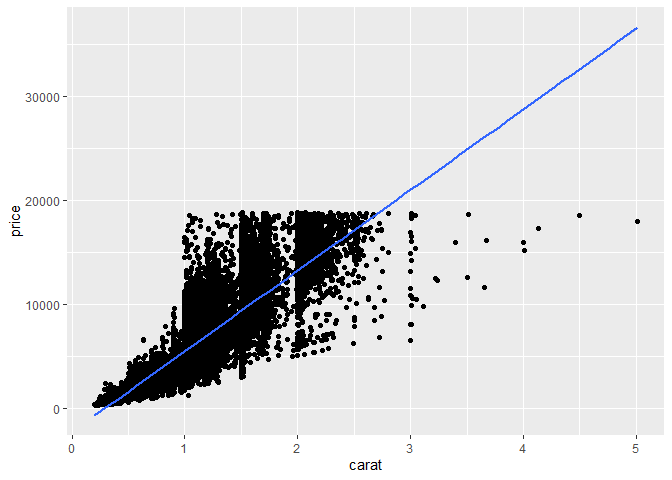
\includegraphics{hw_08_files/figure-latex/unnamed-chunk-5-1.pdf}

\begin{Shaded}
\begin{Highlighting}[]
\CommentTok{#The 'plus' means I am adding "layers" to my ggplot}
\CommentTok{#This is a poorly made scatterplot, so I will make a tab and create another scatterplot. }
\end{Highlighting}
\end{Shaded}

\hypertarget{plots}{%
\section{Plots}\label{plots}}

\hypertarget{scatter-plot}{%
\subsection{Scatter Plot}\label{scatter-plot}}

\begin{Shaded}
\begin{Highlighting}[]
\KeywordTok{ggplot}\NormalTok{(Dec_Jun_wind, }\KeywordTok{aes}\NormalTok{(}\DataTypeTok{x =}\NormalTok{ day, }
                         \DataTypeTok{y =}\NormalTok{ wind_speed)) }\OperatorTok{+}
\StringTok{  }\KeywordTok{geom_point}\NormalTok{(}\DataTypeTok{mapping =} \KeywordTok{aes}\NormalTok{(}\DataTypeTok{color =}\NormalTok{ wind_gust)) }\OperatorTok{+}
\StringTok{  }\KeywordTok{scale_color_distiller}\NormalTok{(}\DataTypeTok{type =} \StringTok{"seq"}\NormalTok{, }
                       \DataTypeTok{palette =} \StringTok{"Greens"}\NormalTok{, }
                       \DataTypeTok{guide =} \KeywordTok{guide_legend}\NormalTok{(}\DataTypeTok{reverse =} \OtherTok{TRUE}\NormalTok{), }
                       \DataTypeTok{direction =} \DecValTok{1}\NormalTok{) }\OperatorTok{+}
\StringTok{  }\KeywordTok{labs}\NormalTok{(}\DataTypeTok{title =} \StringTok{"Wind Speed and Gust on a Given Day In Jun and Dec, 2013"}\NormalTok{, }
       \DataTypeTok{x =} \StringTok{"Day"}\NormalTok{, }
       \DataTypeTok{y =} \StringTok{"Wind Speed (mph)"}\NormalTok{,}
      \DataTypeTok{color =} \StringTok{"Wind Gust (mph)"}\NormalTok{)}
\end{Highlighting}
\end{Shaded}

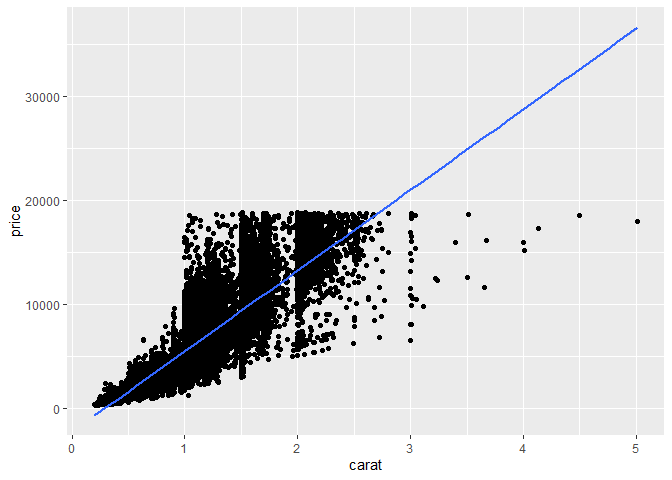
\includegraphics{hw_08_files/figure-latex/unnamed-chunk-6-1.pdf}

\end{document}
